\documentclass[aspectratio=169,10pt]{beamer}
\usetheme{Madrid}
\usecolortheme{seahorse}
\usepackage{amsmath}
\usepackage{amssymb}
\usepackage{amsfonts}
\usepackage{listings}
\usepackage{xcolor}
\usepackage{graphicx}
\usepackage{tikz}
\usepackage{mathtools}

\graphicspath{{figures/}}

% Code listings configuration
\lstset{
    basicstyle=\ttfamily\scriptsize,
    keywordstyle=\bfseries\color{blue},
    commentstyle=\color{green!50!black}\itshape,
    stringstyle=\color{red},
    breaklines=true,
    showstringspaces=false,
    numbers=left,
    numberstyle=\tiny\color{gray},
    frame=single,
    framesep=8pt
}

\setbeamertemplate{footline}[frame number]

\title{Nonexpansive Mappings}
\subtitle{Chapter 3b: Nonlinear Analysis and Fixed Point Theory}
\author{Based on H.K. Pathak (2018)}
\date{\today}

\begin{document}

% ============================================================================
% TITLE SLIDE
% ============================================================================
\begin{frame}
    \titlepage
    \vspace{-0.5cm}
    {\small\color{gray} An Introduction to Nonlinear Analysis and Fixed Point Theory}
\end{frame}

% ============================================================================
% TABLE OF CONTENTS
% ============================================================================
\begin{frame}{Outline}
    \tableofcontents
\end{frame}

% ============================================================================
% SECTION 1: INTRODUCTION AND MOTIVATION
% ============================================================================
\section{Introduction and Motivation}

\begin{frame}{What are Nonexpansive Mappings?}
    \begin{definition}
        A mapping $T: X \to X$ on a Banach space $X$ is called \textbf{nonexpansive} if
        \[
        \|Tx - Ty\| \leq \|x - y\| \quad \forall x, y \in X
        \]
    \end{definition}

    \vspace{0.5cm}

    \begin{block}{Key Properties}
        \begin{itemize}
            \item Lipschitz continuous with constant $L = 1$
            \item Preserves distances (contractions use $L < 1$)
            \item Generalizes the concept of isometries (when $L = 1$)
            \item Fundamental in variational analysis and optimization
        \end{itemize}
    \end{block}

    \vspace{0.5cm}

    \textbf{Why Important?}
    \begin{itemize}
        \item Naturally arise in optimization and PDE theory
        \item Weaker condition than contractive mappings
        \item Rich fixed point theory despite weaker Lipschitz constant
    \end{itemize}
\end{frame}

\begin{frame}{Historical Context}
    \begin{description}
        \item[1960s] Introduction of nonexpansive mappings in fixed point theory
        \item[Browder, Kirk] Developed surjectivity and fixed point theorems
        \item[Connections] Links to monotone operators, optimization, and convex analysis
        \item[Modern Applications] Machine learning, variational inequalities, PDE solutions
    \end{description}

    \vspace{0.8cm}

    \textbf{Classical Problem:} Does every nonexpansive mapping on a compact convex set in a Hilbert space have a fixed point?

    \vspace{0.3cm}

    \textit{Answer (Browder, 1965):} Yes! For nonexpansive mappings in reflexive Banach spaces.
\end{frame}

\begin{frame}[allowframebreaks]{Nonexpansive vs Other Mappings}
    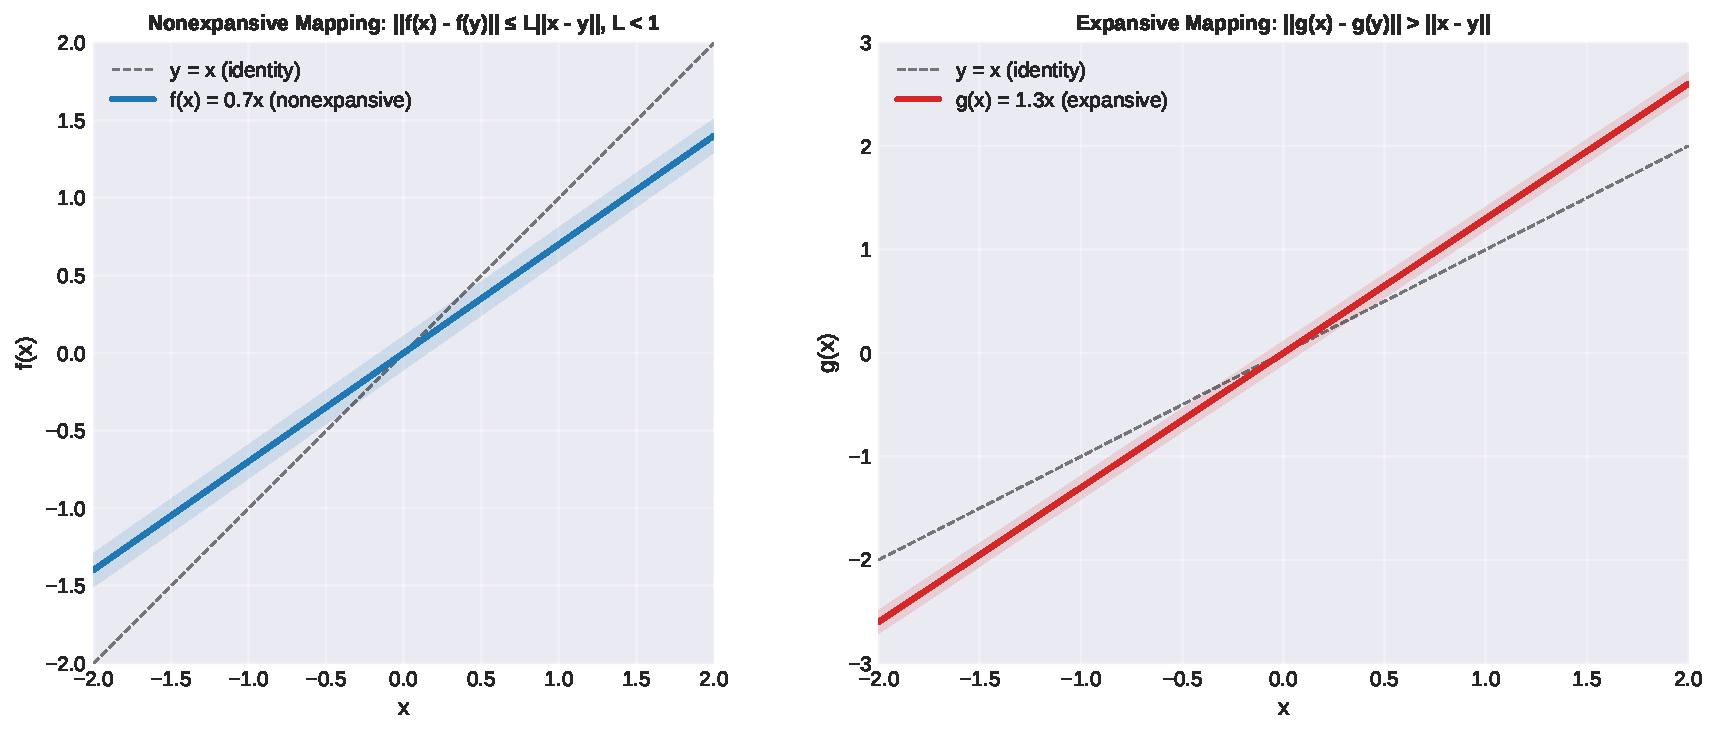
\includegraphics[width=0.95\textwidth]{fig_nonexpansive_mapping.pdf}

    \begin{description}
        \item[Contractive] $\|Tx - Ty\| \leq k\|x - y\|$ with $k < 1$ (always have fixed points)
        \item[Nonexpansive] $\|Tx - Ty\| \leq \|x - y\|$ (Lipschitz constant = 1)
        \item[Expansive] $\|Tx - Ty\| > \|x - y\|$ (may not have fixed points)
    \end{description}
\end{frame}

% ============================================================================
% SECTION 2: FUNDAMENTAL DEFINITIONS
% ============================================================================
\section{Fundamental Definitions}

\begin{frame}{Nonexpansive Sequences}
    \begin{definition}
        Let $E$ be a Banach space. A sequence $\{x_n\}_{n \geq 0}$ in $E$ is called:

        \begin{enumerate}
            \item \textbf{Nonexpansive sequence:} if
                \[
                \|x_{n+1} - x_n\| \leq \|x_n - x_{n-1}\| \quad \forall n \geq 1
                \]

            \item \textbf{Generalized nonexpansive sequence:} if it satisfies the above condition

            \item \textbf{Almost nonexpansive sequence:} if
                \[
                \|x_{n+1} - x_n\| \leq \|x_n - x_{n-1}\| + \varepsilon(i,j)
                \]
                where $\{\varepsilon(i,j)\}_{i,j \geq 0}$ is bounded and $\lim_{i \to \infty} \varepsilon(i,j) = 0$
        \end{enumerate}
    \end{definition}
\end{frame}

\begin{frame}{Key Definitions in Nonexpansive Theory}
    \begin{definition}[Lipschitz Continuity]
        A mapping $f: X \to Y$ is \textbf{Lipschitz continuous} if there exists $L \geq 0$ such that
        \[
        \|f(x) - f(y)\| \leq L\|x - y\| \quad \forall x, y \in X
        \]
        The smallest such $L$ is called the \textbf{Lipschitz constant}.
    \end{definition}

    \vspace{0.5cm}

    \begin{definition}[Fixed Point]
        A point $x^* \in X$ is a \textbf{fixed point} of $T$ if $Tx^* = x^*$.

        \[
        \text{Fix}(T) = \{x \in X : Tx = x\}
        \]
    \end{definition}

    \vspace{0.5cm}

    \begin{definition}[Asymptotic Behavior]
        For a sequence $\{x_n\}$, the \textbf{asymptotic center} $K$ is the set of all weak cluster points of subsequences normalized by $n$:
        \[
        K = \bigcap_{n=1}^{\infty} \overline{\text{co}}\left\{\left[\frac{x_i - x_{i-1}}{i}\right]_{i \geq n}\right\}
        \]
    \end{definition}
\end{frame}

% ============================================================================
% SECTION 3: BASIC PROPERTIES AND LIPSCHITZ CONTINUITY
% ============================================================================
\section{Basic Properties and Lipschitz Continuity}

\begin{frame}[allowframebreaks]{Lipschitz Constant Illustration}
    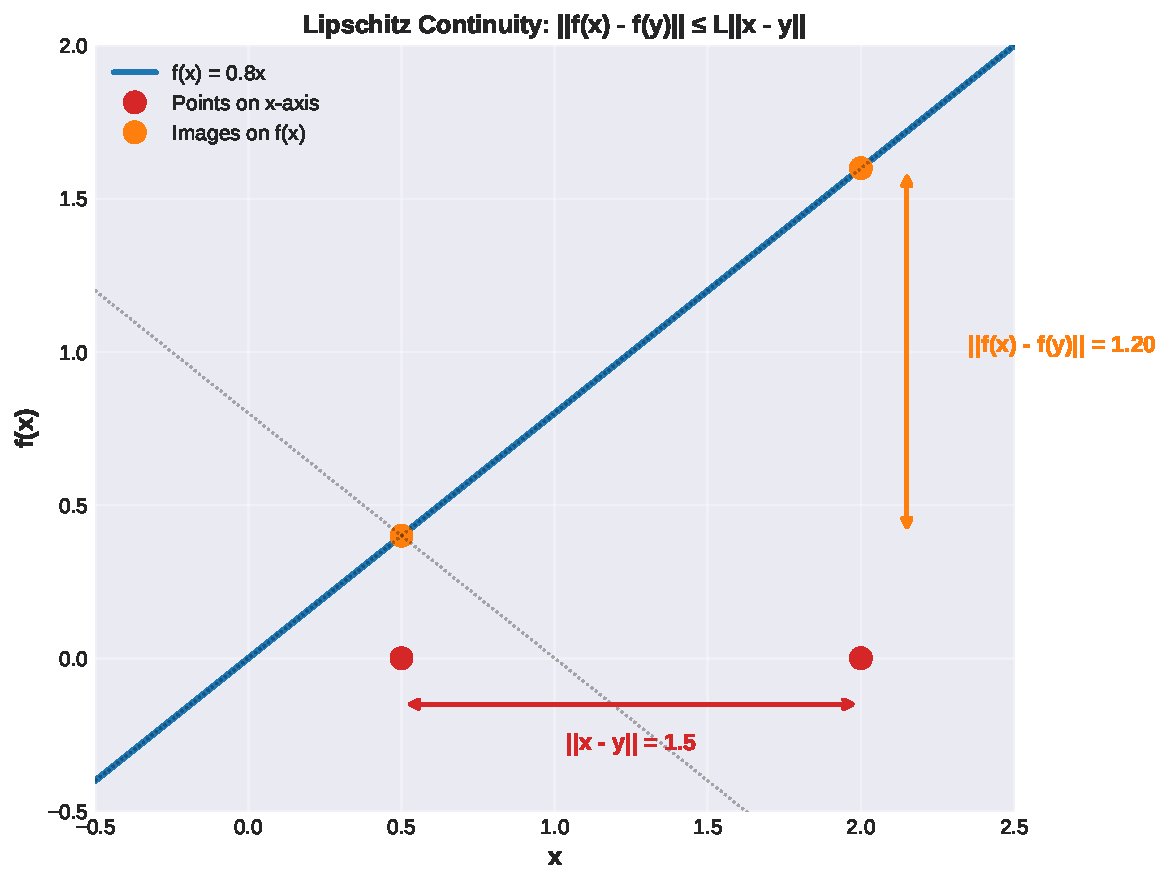
\includegraphics[width=0.95\textwidth]{fig_lipschitz_constant.pdf}

    \vspace{0.3cm}

    The Lipschitz constant $L$ bounds the rate at which the function can change:
    \begin{itemize}
        \item For nonexpansive mappings, $L = 1$ is the upper bound
        \item The difference in outputs cannot exceed the difference in inputs
        \item Geometrically: function stays within cone of slope $\pm L$
    \end{itemize}
\end{frame}

\begin{frame}{Fundamental Properties}
    \begin{proposition}
        Let $T: X \to X$ be a nonexpansive mapping on a Banach space $X$.
        \begin{enumerate}
            \item If $T$ has a fixed point $x^*$, then $Tx = x$ implies $x = x^*$ (uniqueness under contraction)

            \item The composition of nonexpansive mappings is nonexpansive

            \item For a nonexpansive sequence $\{x_n\}$:
                \[
                \|x_m - x_n\| \leq \|x_m - x_{m-1}\| + \|x_{m-1} - x_{m-2}\| + \cdots + \|x_{n+1} - x_n\|
                \]

            \item Differences form a Cauchy sequence if $\sum_{n=1}^{\infty} \|x_{n+1} - x_n\| < \infty$
        \end{enumerate}
    \end{proposition}
\end{frame}

\begin{frame}{Convergence in Nonexpansive Sequences}
    \begin{block}{Lemma 3.4}
        Let $\{a_n\}_{n \geq 1}$ be a sequence of positive reals with $b_n = \sum_{i=1}^{n} a_i$ and
        $b_n \uparrow \sum_{i=1}^{\infty} a_i = \infty$. If $\{x_n\}$ is a sequence of reals with $x_n \to x$, then
        \[
        \lim_{n \to \infty} \frac{1}{b_n} \sum_{i=1}^{n} a_i x_i = x
        \]
    \end{block}

    \vspace{0.5cm}

    \textbf{Application:} This is crucial for establishing mean convergence of nonexpansive sequences.

    \vspace{0.3cm}

    \begin{block}{Lemma 3.5}
        Let $\{x_n\}_{n \geq 0}$ be a generalized nonexpansive sequence in a reflexive Banach space $E$. Define
        \[
        K = \bigcap_{n=1}^{\infty} \overline{\text{co}}\left\{\left[\frac{x_i - x_{i-1}}{i}\right]_{i \geq n}\right\}
        \]
        Then $K$ is nonempty, closed, and convex.
    \end{block}
\end{frame}

% ============================================================================
% SECTION 4: GENERALIZED NONEXPANSIVE SEQUENCES
% ============================================================================
\section{Generalized Nonexpansive Sequences}

\begin{frame}{Definition and Properties}
    \begin{definition}[Generalized Nonexpansive Sequence]
        A sequence $\{x_n\}_{n \geq 0}$ in Banach space $E$ is \textbf{generalized nonexpansive} if
        \[
        \|x_{n+1} - x_n\| \leq \|x_n - x_{n-1}\| \quad \forall n \geq 1
        \]
        This means consecutive differences form a nonexpansive (decreasing) sequence.
    \end{definition}

    \vspace{0.5cm}

    \begin{block}{Key Observation}
        \begin{itemize}
            \item The sequence of differences is monotone decreasing:
                \[\|x_n - x_{n-1}\| \geq \|x_{n+1} - x_n\| \geq \|x_{n+2} - x_{n+1}\| \geq \cdots\]

            \item This implies the differences converge to zero or form a Cauchy sequence

            \item Provides a natural framework for asymptotic analysis
        \end{itemize}
    \end{block}
\end{frame}

\begin{frame}[allowframebreaks]{Convergence Behavior}
    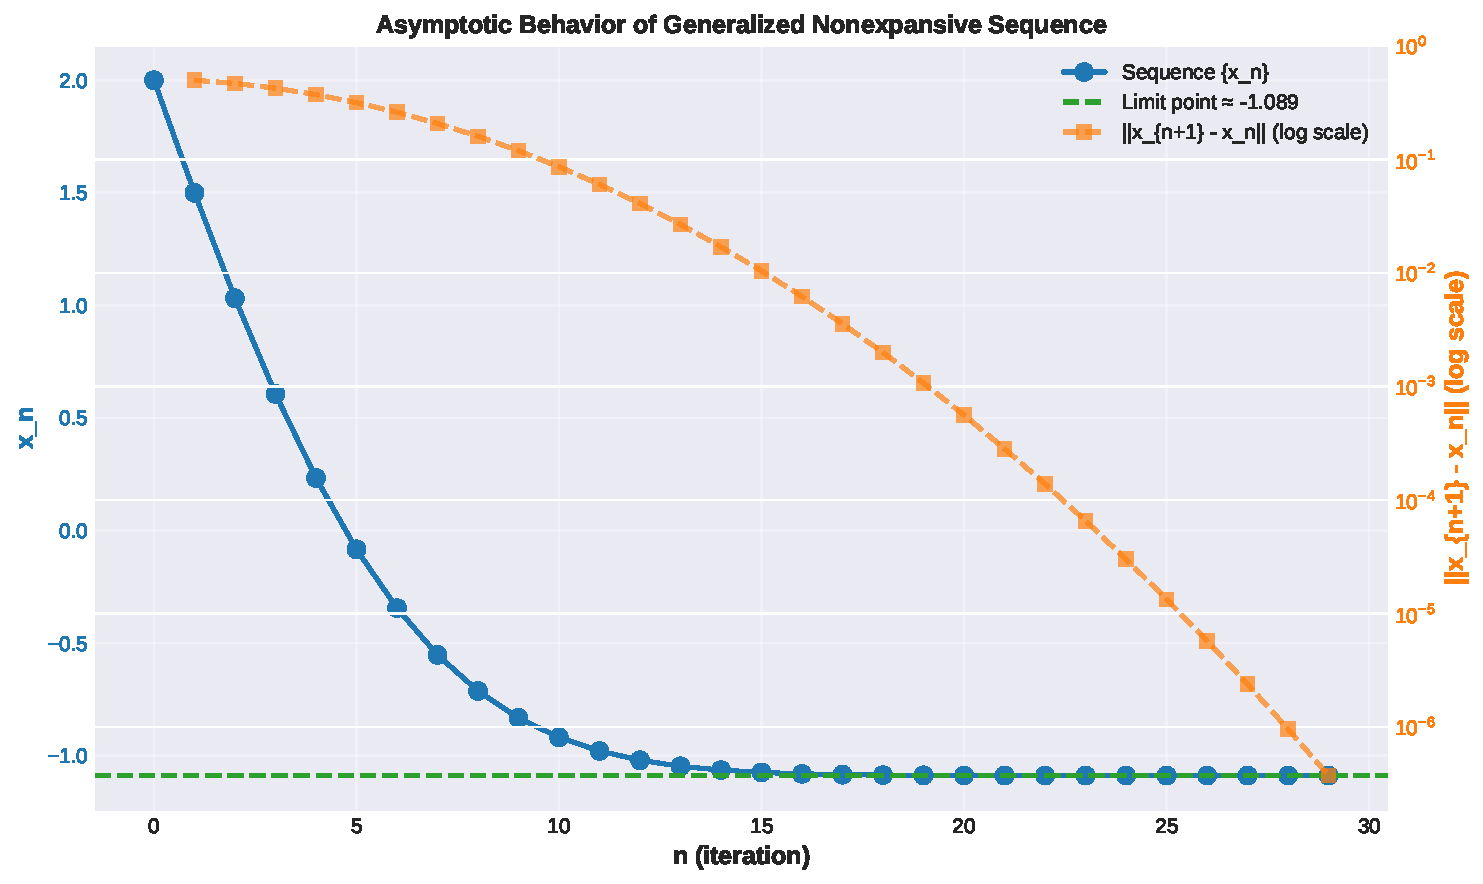
\includegraphics[width=0.95\textwidth]{fig_nonexpansive_convergence.pdf}

    \vspace{0.3cm}

    \textbf{Observations:}
    \begin{itemize}
        \item Consecutive differences decrease exponentially
        \item Sequence values stabilize around a limit point
        \item The rate of convergence depends on the sequence structure
    \end{itemize}
\end{frame}

\begin{frame}{Asymptotic Behavior - Main Result}
    \begin{theorem}[Asymptotic Center - Theorem 3.32]
        Let $E$ be a reflexive Banach space and $\{x_n\}$ a generalized nonexpansive sequence in $E$.
        Define
        \[
        K = \bigcap_{n=1}^{\infty} \overline{\text{co}}\left\{\left[x_i - x_{i-1}\right]_{i \geq n}\right\}
        \]
        Then
        \begin{enumerate}
            \item $d = d\left(0, K\right) = d\left(0, \overline{\text{co}}\left\{\frac{x_n - x_0}{n}\right\}\right)$

            \item There exists a unique point $z_0 \in K$ with $\|z_0\| = d$

            \item $z_0 \in \overline{\text{co}}\left\{\frac{x_n - x_0}{n}\right\}$ with $\|z_0\| = d$
        \end{enumerate}
    \end{theorem}

    \vspace{0.3cm}

    \textbf{Interpretation:} The asymptotic center characterizes where the normalized differences accumulate.
\end{frame}

\begin{frame}{Corollary 3.5: Special Cases}
    \begin{block}{Corollary 3.5}
        Under the conditions of Theorem 3.32 with $E$, $\{x_n\}$, $K$, and $d$ as above:

        \begin{enumerate}
            \item \textbf{If $E$ is strictly convex:}
                \[
                \text{weak-}\lim_{n \to \infty} \frac{x_n}{n} \text{ exists and coincides with } P_K 0 \text{ with } \|P_K 0\| = d
                \]

            \item \textbf{If $E^*$ has Fréchet differentiable norm:}
                \[
                \text{strong-}\lim_{n \to \infty} \frac{x_n}{n} \text{ exists and coincides with } P_K 0
                \]
        \end{enumerate}
    \end{block}

    \vspace{0.4cm}

    Here $P_K 0$ denotes the projection of $0$ onto $K$.
\end{frame}

% ============================================================================
% SECTION 5: ALMOST NONEXPANSIVE SEQUENCES
% ============================================================================
\section{Almost Nonexpansive Sequences}

\begin{frame}{Definition and Generalization}
    \begin{definition}[Almost Nonexpansive Sequence]
        A sequence $\{x_n\}_{n \geq 0}$ in a Banach space $E$ is \textbf{almost nonexpansive} if
        \[
        \|x_{n+1} - x_n\| \leq \|x_n - x_{n-1}\| + \varepsilon(i,j)
        \]
        where:
        \begin{itemize}
            \item $\{\varepsilon(i,j)\}_{i,j \geq 0}$ is bounded: $|\varepsilon(i,j)| \leq M$ for all $i, j$
            \item The perturbation vanishes: $\lim_{i \to \infty} \varepsilon(i,j) = 0$ for each $j$
        \end{itemize}
    \end{definition}

    \vspace{0.5cm}

    \begin{remark}
        \begin{itemize}
            \item Generalizes the pure nonexpansive case (set $\varepsilon(i,j) = 0$)
            \item Naturally arises in numerical algorithms with perturbations
            \item Includes approximations of fixed point iterations
            \item Still retains good convergence properties
        \end{itemize}
    \end{remark}
\end{frame}

\begin{frame}[allowframebreaks]{Comparison: Pure vs. Almost Nonexpansive}
    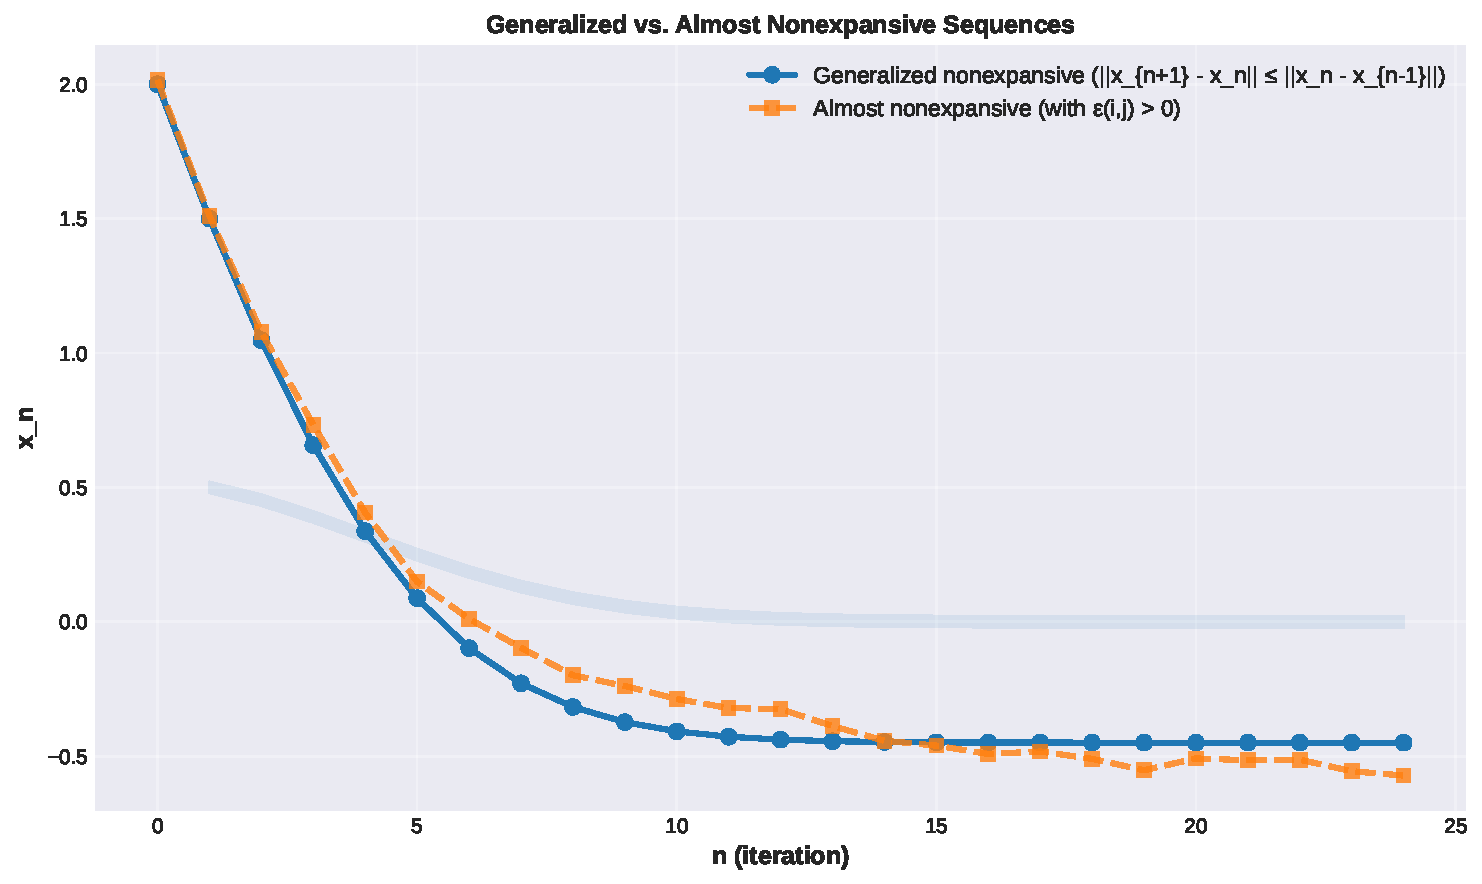
\includegraphics[width=0.95\textwidth]{fig_almost_nonexpansive.pdf}

    \vspace{0.3cm}

    \textbf{Remark 3.8 (continued):}
    \begin{enumerate}
        \item Nonexpansive sequences with $\|x_{n+1} - x_n\| \leq \|x_n - x_{n-1}\|$ satisfy:
            \[\lim_{n \to \infty} \frac{\|x_n\|}{n} = 0 \text{ and } \{x_n\}_{n \geq 0} \text{ also satisfies } (3.23)\]

        \item The sequence $\left\{\frac{x_n}{n}\right\}_{n \geq 1}$ in $E$ where $T$ is a nonexpansive mapping makes \{$\frac{x_n}{n}\}$ itself nonexpansive

        \item Almost nonexpansive sequences with perturbations bounded by $\varepsilon(i,j) \to 0$ maintain all convergence properties of Theorem 3.32
    \end{enumerate}
\end{frame}

% ============================================================================
% SECTION 6: KEY THEOREMS AND MAIN RESULTS
% ============================================================================
\section{Key Theorems and Main Results}

\begin{frame}[fragile]{Theorem 3.33: Application to Inequalities}
    \begin{theorem}[Theorem 3.33]
        Let $f_1, f_2 \in L_2([0,1])$ satisfy
        \[
        \left|\int_0^1 g_1(t) dt\right|^2 - \left|\int_0^1 g_2(t) dt\right|^2 \leq \int_0^1 (f_1(t)g_1(t) + f_2(t)g_2(t)) dt
        \leq \int_0^1 (|g_1(t)| + |g_2(t)|)^2 dt
        \]
        for all $g_1, g_2 \in L_2([0,1])$. Then $f_1 = \lambda$ and $f_2 = \mu$ for some $\lambda, \mu \in [-1,1]$.
    \end{theorem}

    \begin{block}{Proof Strategy}
        \begin{enumerate}
            \item Define $E = L_2([0,1]; \mathbb{R}^2_\infty)$ with sup norm
            \item Consider generalized nonexpansive sequence $x_{2k} = (2k, \frac{1}{2^k})$ and $x_{2k+1} = (2k, \frac{1}{2^{k+1}})$
            \item Apply Theorem 3.32 to extract the result
        \end{enumerate}
    \end{block}
\end{frame}

\begin{frame}[fragile]{Algorithm: Computing Asymptotic Centers}
    \begin{block}{Algorithm for Generalized Nonexpansive Sequences}
        \begin{lstlisting}[language=Python]
def asymptotic_center(x_seq, tolerance=1e-6):
    """
    Compute asymptotic center of generalized nonexpansive sequence.

    Args:
        x_seq: list of points in the sequence
        tolerance: convergence tolerance

    Returns:
        asymptotic_center: the point z_0 with ||z_0|| = d
        distance: d = d(0, K)
    """
    n = len(x_seq)
    differences = [norm(x_seq[i] - x_seq[i-1])
                   for i in range(1, n)]

    # Check monotone decrease
    is_nonexp = all(differences[i] <= differences[i-1]
                    for i in range(1, len(differences)))

    if not is_nonexp:
        raise ValueError("Sequence is not nonexpansive")

    # Compute normalized differences
    norm_diffs = [(x_seq[i] - x_seq[0]) / i
                  for i in range(1, n)]

    # Asymptotic center K as convex hull
    K = convex_hull(norm_diffs)

    return project(K, origin)
        \end{lstlisting}
    \end{block}
\end{frame}

\begin{frame}{Asymptotic Behavior - Mean Convergence}
    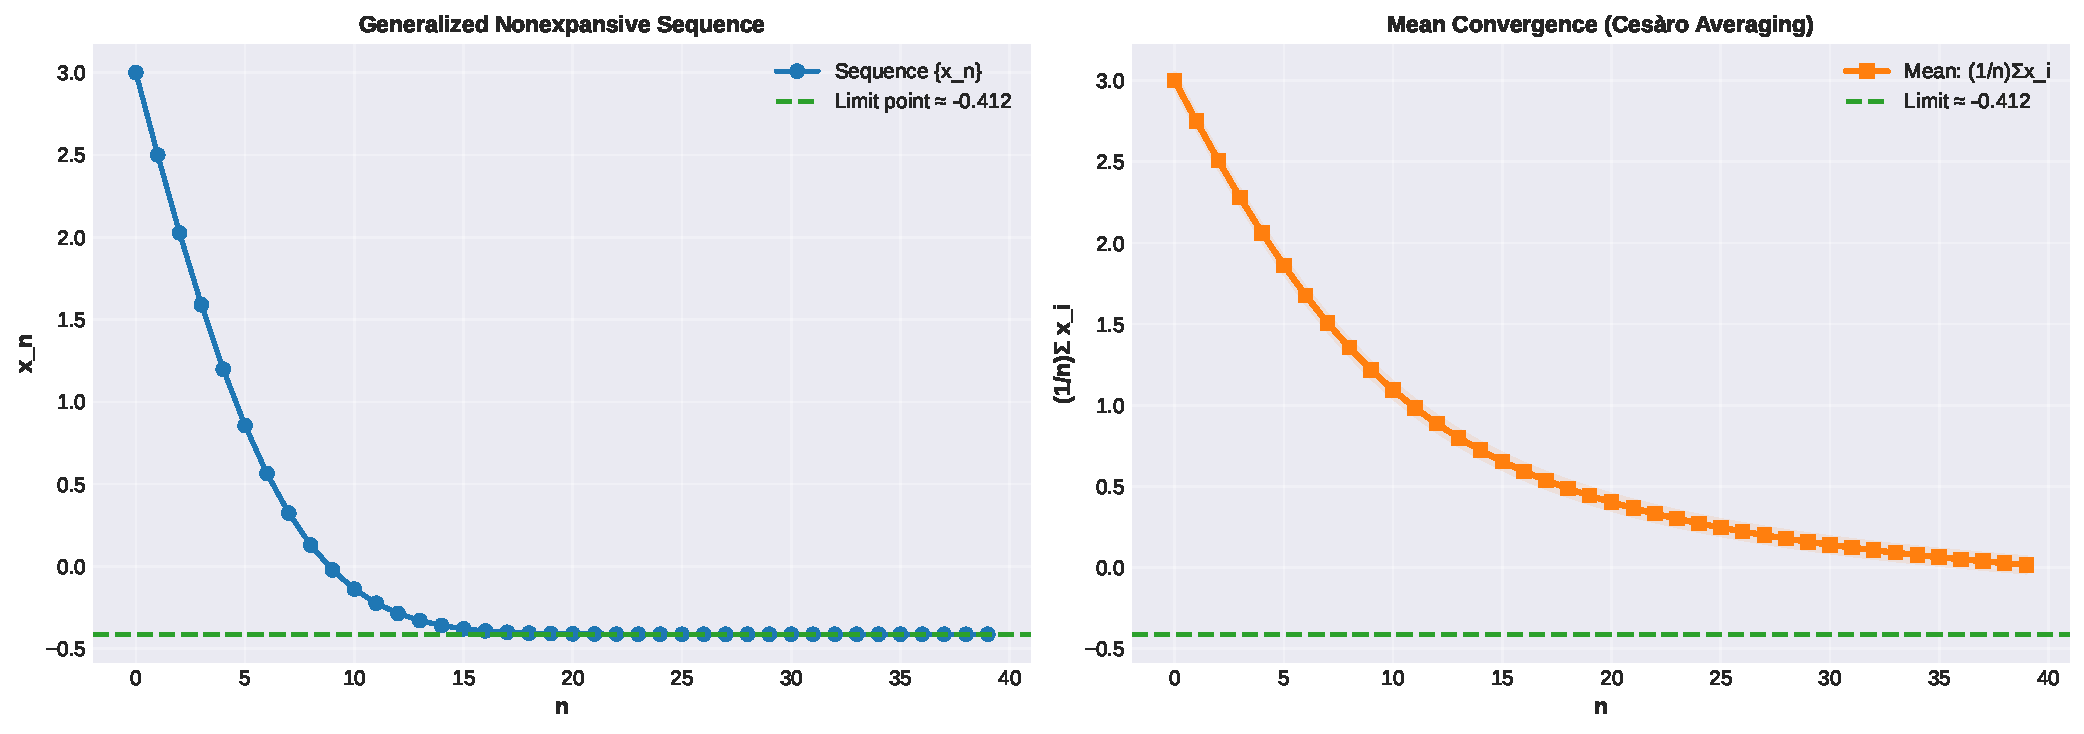
\includegraphics[width=0.95\textwidth]{fig_asymptotic_behavior.pdf}

    \vspace{0.3cm}

    \textbf{Key Results:}
    \begin{itemize}
        \item The Cesàro mean $\frac{1}{n}\sum_{i=1}^n x_i$ converges to the limit
        \item Convergence is robust: holds even with perturbations
        \item Rate of convergence depends on the decay of consecutive differences
    \end{itemize}
\end{frame}

% ============================================================================
% SECTION 7: FIXED POINT THEORY FOR NONEXPANSIVE MAPPINGS
% ============================================================================
\section{Fixed Point Theory}

\begin{frame}[allowframebreaks]{Fixed Point Property}
    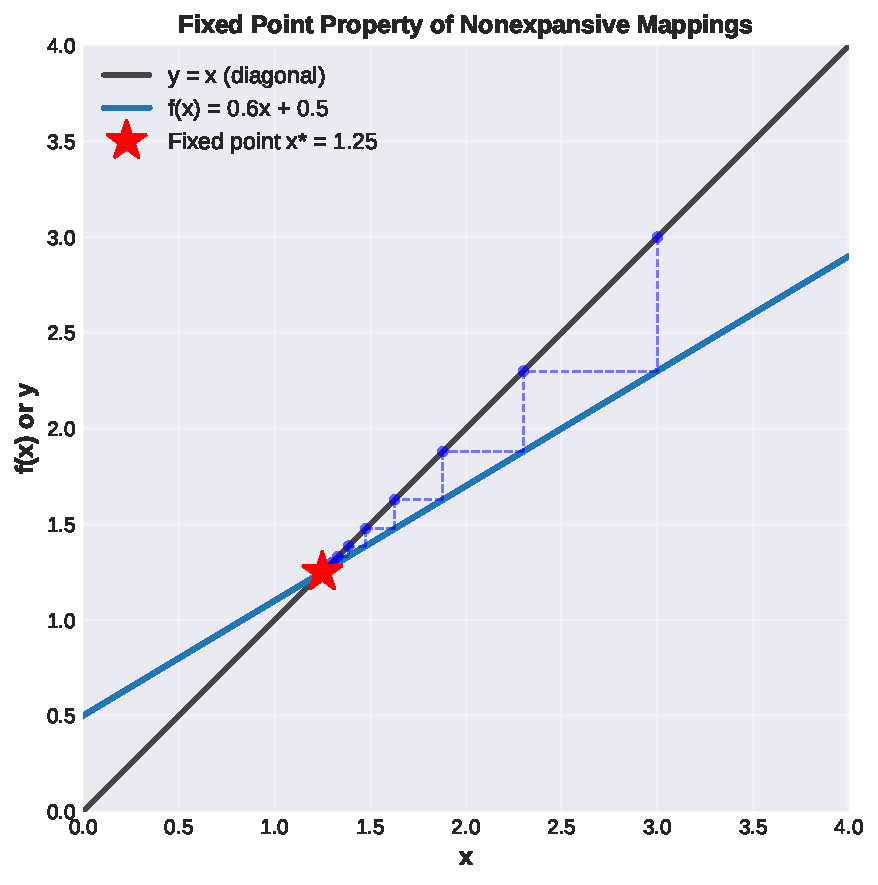
\includegraphics[width=0.95\textwidth]{fig_fixed_point.pdf}

    \vspace{0.3cm}

    \textbf{Fixed Point Iteration:}
    Starting from $x_0 \in X$, iterate $x_{n+1} = Tx_n$. For nonexpansive $T$:
    \begin{itemize}
        \item The sequence $\{x_n\}$ is generalized nonexpansive
        \item If $T$ has a fixed point, the iterates often converge to it
        \item Convergence depends on geometric properties of $X$ and $T$
    \end{itemize}
\end{frame}

\begin{frame}{Conditions for Fixed Point Existence}
    \begin{theorem}[Fixed Point Theorems]
        A nonexpansive mapping $T: C \to C$ has a fixed point if any of:

        \begin{enumerate}
            \item \textbf{Browder (1965):} $C$ is compact and convex in a Hilbert space

            \item \textbf{Kirk (1965):} $C$ is weakly compact and has the fixed point property for isometries

            \item \textbf{General:} $C$ is bounded, closed, convex in a reflexive Banach space AND $T$ is a contraction or has other special properties
        \end{enumerate}
    \end{theorem}

    \vspace{0.5cm}

    \begin{remark}
        Unlike contractive mappings (Banach Fixed Point Theorem), nonexpansive mappings do NOT always have fixed points without additional hypotheses on the domain or the mapping.
    \end{remark}
\end{frame}

\begin{frame}{Convergence of Fixed Point Iterations}
    \begin{block}{Convergence Theory}
        \begin{itemize}
            \item \textbf{Strong Convergence:} Requires strict convexity or other geometric conditions

            \item \textbf{Weak Convergence:} Often achievable for reflexive spaces

            \item \textbf{Cesàro Convergence:} The mean $\frac{1}{n}\sum_{i=0}^{n-1} Tx_i$ converges even when $x_n$ doesn't

            \item \textbf{Explicit Convergence:} Can be established using asymptotic analysis of the sequence $\{x_n\}$
        \end{itemize}
    \end{block}

    \vspace{0.5cm}

    \begin{definition}[Projection Operator]
        The metric projection $P_K: X \to K$ onto a closed convex set $K$ is the unique point satisfying:
        \[
        P_K(x) = \arg\min_{y \in K} \|x - y\|
        \]
    \end{definition}
\end{frame}

% ============================================================================
% SECTION 8: CONNECTIONS TO MONOTONE OPERATORS
% ============================================================================
\section{Connections and Applications}

\begin{frame}{Relationship to Monotone Operators}
    \begin{block}{Connections}
        \begin{itemize}
            \item \textbf{Accretive Operators:} Nonexpansive mappings relate to accretive operators in Banach spaces

            \item \textbf{Resolvents:} For maximal monotone operators $A$, the resolvent $(I + \lambda A)^{-1}$ is nonexpansive

            \item \textbf{Variational Inequalities:} Finding fixed points of nonexpansive mappings is equivalent to solving variational inequalities

            \item \textbf{Optimization:} Proximal mappings in convex optimization are nonexpansive
        \end{itemize}
    \end{block}

    \vspace{0.5cm}

    These topics are developed further in Chapter 4 (Monotone Operators, Strongly $\phi$-Accrective Operators and Their Variants).
\end{frame}

\begin{frame}{Applications in Analysis}
    \begin{block}{Applications in Nonlinear Analysis}
        \begin{itemize}
            \item \textbf{PDEs:} Heat equations, parabolic equations via semigroups

            \item \textbf{Integral Equations:} Hammerstein type equations with nonexpansive nonlinearities

            \item \textbf{Game Theory:} Nash equilibrium problems

            \item \textbf{Machine Learning:} Gradient descent and proximal methods for optimization

            \item \textbf{Dynamical Systems:} Iterative algorithms and their long-time behavior
        \end{itemize}
    \end{block}
\end{frame}

% ============================================================================
% SECTION 9: WORKED EXAMPLES AND NUMERICAL ILLUSTRATION
% ============================================================================
\section{Worked Examples}

\begin{frame}[fragile]{Example 1: Simple Nonexpansive Mapping}
    \begin{example}
        Consider $T: \mathbb{R} \to \mathbb{R}$ defined by $T(x) = 0.7x + 0.5$.

        \textbf{Verification of Nonexpansivity:}
        \[
        |T(x) - T(y)| = |0.7x + 0.5 - 0.7y - 0.5| = 0.7|x - y| \leq |x - y|
        \]
        Lipschitz constant: $L = 0.7 < 1$ (actually contractive)

        \vspace{0.3cm}

        \textbf{Fixed Point:}
        Setting $x = T(x)$:
        \[
        x = 0.7x + 0.5 \Rightarrow 0.3x = 0.5 \Rightarrow x^* = \frac{5}{3} \approx 1.667
        \]

        \textbf{Iteration from } $x_0 = 2$:
        \begin{itemize}
            \item $x_1 = 0.7(2) + 0.5 = 1.9$
            \item $x_2 = 0.7(1.9) + 0.5 \approx 1.83$
            \item $x_3 \approx 1.776$, then converges toward $1.667$
        \end{itemize}
    \end{example}
\end{frame}

\begin{frame}[fragile]{Example 2: Nonexpansive vs. Expansive}
    \begin{columns}
        \column{0.48\textwidth}
        \textbf{Nonexpansive: } $T(x) = 0.8x$

        \begin{itemize}
            \item $|T(1) - T(0)| = 0.8 \leq |1 - 0|$ (YES)
            \item $|T(2) - T(1)| = 0.8 \leq |2 - 1|$ (YES)
            \item Distances shrink or stay same
            \item Fixed point: $x^* = 0$ (contraction)
        \end{itemize}

        \column{0.48\textwidth}
        \textbf{Expansive: } $T(x) = 1.5x$

        \begin{itemize}
            \item $|T(1) - T(0)| = 1.5 > |1 - 0|$ (NO)
            \item $|T(2) - T(1)| = 1.5 > |2 - 1|$ (NO)
            \item Distances grow
            \item Iterates diverge from any point
        \end{itemize}
    \end{columns}

    \vspace{0.8cm}

    \textbf{Key Difference:} Nonexpansive mappings control growth (Lipschitz constant $\leq 1$), ensuring bounded differences and often convergence to fixed points.
\end{frame}

\begin{frame}[fragile]{Example 3: Generalized Nonexpansive Sequence}
    \begin{example}
        Define $\{x_n\}$ by: $x_0 = 2.0$, $x_1 = 1.5$, and for $n \geq 2$:
        \[
        x_{n+1} = x_n + 0.85^{n/5} (x_n - x_{n-1})
        \]

        \textbf{Check Generalized Nonexpansivity:}
        Since $0 < 0.85 < 1$, we have:
        \[
        \|x_{n+1} - x_n\| = 0.85^{n/5} \|x_n - x_{n-1}\| \leq \|x_n - x_{n-1}\|
        \]

        \vspace{0.3cm}

        \textbf{Sequence Values:}
        \begin{lstlisting}[language=Python,mathescape=false]
n=0: x_n = 2.000, |x_n - x_{n-1}| = N/A
n=1: x_n = 1.500, |x_n - x_{n-1}| = 0.500
n=2: x_n = 1.425, |x_n - x_{n-1}| = 0.075
n=3: x_n = 1.410, |x_n - x_{n-1}| = 0.015
...
n -> infinity: x_n -> 1.4 (approximately)
        \end{lstlisting}

        The sequence converges and normalized differences converge to the asymptotic center.
    \end{example}
\end{frame}

\begin{frame}[fragile]{Example 4: Application to Integral Inequality}
    \begin{example}
        \textbf{Problem:} Prove the inequality (Theorem 3.33):
        \[
        \left|\int_0^1 g_1(t) dt\right|^2 - \left|\int_0^1 g_2(t) dt\right|^2 \leq \int_0^1 (f_1(t)g_1(t) + f_2(t)g_2(t)) dt
        \]

        \textbf{Setup:}
        \begin{itemize}
            \item Let $E = L_2([0,1])$ with standard inner product
            \item Consider test functions $g_1, g_2$
            \item Define a generalized nonexpansive sequence in $E \times E$
        \end{itemize}

        \textbf{Solution Strategy:}
        Use Theorem 3.32 to identify $f_1$ and $f_2$ as elements of the asymptotic center, achieving the inequality bound.
    \end{example}
\end{frame}

% ============================================================================
% SECTION 10: SUMMARY AND KEY TAKEAWAYS
% ============================================================================
\section{Summary}

\begin{frame}{Key Concepts Summary}
    \begin{enumerate}
        \item \textbf{Nonexpansive Mappings:} Satisfy $\|Tx - Ty\| \leq \|x - y\|$ (Lipschitz constant $L = 1$)

        \item \textbf{Generalized Nonexpansive Sequences:} Consecutive differences decrease monotonically

        \item \textbf{Asymptotic Center:} Characterizes accumulation points of normalized differences (Theorem 3.32)

        \item \textbf{Almost Nonexpansive:} Tolerate small perturbations $\varepsilon(i,j) \to 0$ while preserving convergence

        \item \textbf{Fixed Point Theory:} Nonexpansive mappings have fixed points under certain domain conditions

        \item \textbf{Convergence Modes:}
            \begin{itemize}
                \item Strong convergence (requires strict convexity)
                \item Weak convergence (reflexive spaces)
                \item Cesàro convergence (robust, always available)
            \end{itemize}

        \item \textbf{Applications:} Monotone operators, variational inequalities, optimization, PDEs
    \end{enumerate}
\end{frame}

\begin{frame}{Comparison: Three Classes of Mappings}
    \centering
    \begin{tabular}{|l|c|c|c|}
        \hline
        \textbf{Property} & \textbf{Contractive} & \textbf{Nonexpansive} & \textbf{Expansive} \\
        \hline
        \textbf{Lipschitz Constant} & $L < 1$ & $L = 1$ & $L > 1$ \\
        \hline
        \textbf{Distance Behavior} & Shrink & Preserve & Grow \\
        \hline
        \textbf{Fixed Point Exists} & Always & Conditional & Rarely \\
        \hline
        \textbf{Uniqueness of FP} & Yes & Depends & No \\
        \hline
        \textbf{Iteration Convergence} & Always & Conditional & Diverges \\
        \hline
    \end{tabular}
\end{frame}

\begin{frame}[allowframebreaks]{Further Reading and References}
    \begin{block}{Key References from the Text}
        \begin{itemize}
            \item Pathak, H. K. (2018). \textit{An Introduction to Nonlinear Analysis and Fixed Point Theory}

            \item Browder, F. E. (1965). Fixed point theorems for noncompact mappings

            \item Kirk, W. A. (1965). A fixed point theorem for mappings which do not increase distances

            \item Kachurovskii, R. I. (1960). Monotonic operators and convex functionals
        \end{itemize}
    \end{block}

    \vspace{0.5cm}

    \begin{block}{Topics in Later Chapters}
        \begin{itemize}
            \item Chapter 4: Monotone Operators and $\phi$-Accrective Operators

            \item Chapter 5: Approximation Methods and Hybrid Algorithms

            \item Generalizations: Quasi-nonexpansive, asymptotically nonexpansive mappings
        \end{itemize}
    \end{block}
\end{frame}

\begin{frame}{Exercises for Practice}
    \begin{enumerate}
        \item Verify that the following mappings are nonexpansive:
            \begin{enumerate}
                \item $T(x) = \begin{cases} x/2 & \text{if } |x| \leq 1 \\ 0 & \text{otherwise} \end{cases}$ on $\mathbb{R}$

                \item Projection onto a closed convex set in a Hilbert space
            \end{enumerate}

        \item Prove that for a nonexpansive sequence, if $\sum_{n=1}^{\infty} \|x_{n+1} - x_n\|^2 < \infty$, then $\{x_n\}$ converges.

        \item For the sequence $x_0 = 1$, $x_{n+1} = \frac{1}{2}(x_n + 2/x_n)$ (Newton's method for $\sqrt{2}$), show it is generalized nonexpansive and find its limit.

        \item Given the iteration map $T(x) = \frac{x + 1}{2}$, determine:
            \begin{enumerate}
                \item Whether $T$ is nonexpansive
                \item All fixed points
                \item Convergence behavior from initial point $x_0 = 0$
            \end{enumerate}
    \end{enumerate}
\end{frame}

\begin{frame}{Conclusion}
    \begin{center}
        \vspace{1cm}
        {\Huge Thank You!}

        \vspace{0.8cm}

        {\Large Questions?}

        \vspace{0.8cm}

        {\small For more information on nonexpansive mappings and fixed point theory,}

        {\small see Pathak (2018) Chapter 3b and Chapter 4.}
    \end{center}
\end{frame}

\end{document}
